\section{Introduction}

\subsection{Motivation}
% ======================================================================
% Motivation aka. "Why is what we do important?"
%
% First of all: What do we do?
% - We propose a better UQ method for FINN
%
% So I need to say why UQ is important, why FINN is a good method to build on and why the previous method is bad.
%
% But instead of saying why UQ is important in general, I should say why it is important in the context of this work.
%
% So the structure is probably as follows:
% - Context of this work
% - Why FINN is a good method for this
%     - previous methods e.g. model diffusion-sorption with sorption isotherms that are only valid for some conditions
%     - FINN is a physics-aware data-based learning method that does not have these constraints and that can learn various parts of the process and additionally provides interpretable results.
% - Why UQ is imporant here
% - What the previous method was (Bayes NN) and why it is bad (can be inaccurate and computationally expensive)
% - So these limits should be addressed by this work
%
% Main message: Why **efficient** UQ is imporant here
% --------------------------

Understanding and predicting the transport of contaminants in groundwater is paramount for effective environmental remediation and protection. Traditional modeling approaches have been shown to be more inaccurate and less generalizable \cite{finn} than machine learning based approaches. % TODO: I do not like this

The Finite Volume Neural Network (FINN) \cite{finn} offers a promising alternative, leveraging a physics-aware, data-driven approach to learn various parts of the physical process directly from experimental data. This allows for greater flexibility and interpretability compared to traditional methods. However, with the additional complexity, the propagation of uncertainty in the data through the entire process up to the output becomes more challenging. But efficient and reliable uncertainty quantification (UQ) is crucial for determining the confidence in predicted contaminant transport. Existing UQ methods for FINN, such as Bayesian Neural Networks with Markov Chain Monte Carlo (MCMC) sampling \cite{bardenet2017markov}, can be computationally demanding, limiting their practical applicability. This work addresses these limitations by proposing computationally efficient UQ methods for FINN, enabling faster and more reliable uncertainty estimation for contaminant transport predictions.


\subsection{Background}
The transport of contaminants in groundwater is a complex process that involves various physical and chemical interactions. One crucial aspect is diffusion-sorption, where contaminants dissolved in groundwater can interact with the solid phase of the porous medium, such as clay, leading to sorption and desorption processes. This interaction significantly affects the migration and fate of contaminants.

Traditional approaches for modeling contaminant transport rely on numerical solutions of partial differential equations (PDEs) that describe the physical processes. These PDEs often involve parameters that are difficult to measure directly, necessitating the development of parametric models based on physical principles and specific assumptions.
One key parameter in these models is the retardation factor, $R(c)$, which quantifies the effect of sorption on contaminant transport. Sorption, the process by which contaminants attach to the solid phase of the porous medium, can significantly influence the rate and extent of contaminant migration. The retardation factor is typically a function of the contaminant concentration, $c$, and depends on the specific interaction between the contaminant and the soil properties.
A common parametric model for defining $R(c)$ are sorption isotherms. Among the most frequently used are the linear, Freundlich, and Langmuir isotherms \cite{finn} (see Figure \vref{fig:parametric_isotherms}).

Determining the retardation factor from concentration data is an inverse problem. Instead of directly solving the PDE with known parameters, the goal is to infer the unknown retardation factor function ($R(c)$) from observed concentration data. This inverse problem is challenging due to the limited availability and potential noise in the data, as well as the complexity of the underlying sorption processes. Even without noise, uniqueness is not guaranteed for implicit equations. To date, we are not aware of any studies that have mathematically or empirically investigated the uniqueness of the retardation factor for the diffusion-sorption PDE given concentration data and boundary conditions. Understanding the uniqueness of the retardation factor is crucial because it significantly impacts the assessment of uncertainty. If multiple mathematically exact solutions exist, then differences between two solutions obtained by the inverse solver cannot be attributed to uncertainties in the data alone, but may reflect inherent non-uniqueness in the problem itself.

Recent advances like physics-informed neural networks in ML have opened up new possibilities for modeling complex physical systems, including contaminant transport. ML-based approaches can learn intricate relationships from data, offering potential advantages over traditional methods in terms of accuracy, flexibility, and generalizability. FINN \cite{finn} is a physics-informed ML approach that combines the strengths of traditional numerical methods with the adaptability of neural networks. FINN leverages the finite volume method to discretize the governing PDE and employs neural networks to learn the unknown or uncertain components, such as the retardation factor. This allows FINN to incorporate physical constraints and conservation laws while simultaneously learning from data.

While FINN has shown promising results in modeling contaminant transport, quantifying the uncertainty associated with its predictions remains a challenge. Existing UQ methods for FINN, such as BNNs with MCMC sampling, can be computationally demanding, limiting their practical applicability. This motivates the development of more efficient UQ methods for FINN, which is the focus of this study. Our goal is to develop computationally efficient UQ methods for estimating the uncertainty in the retardation factor predicted by FINN, enabling faster and more reliable assessment of contaminant transport predictions.

\begin{figure}[h]
    \centering
    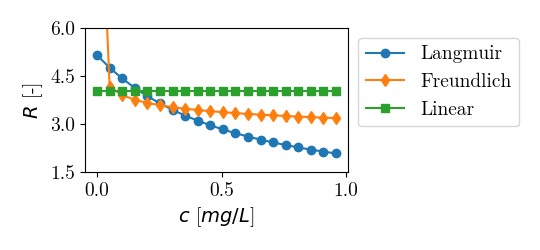
\includegraphics{figs/parametric_isotherms.png}
    \caption{Parametric sorption isotherms for the set of parameters used in Section \vref{sec:TODO}.}
    \label{fig:parametric_isotherms}
\end{figure}


\subsection{Contributions of this Work}
This study addresses UQ in the FINN framework when applied to a diffusion-sorption process. We begin with an empirical analysis of the uniqueness of the retardation factor, which is a crucial step for interpreting the FINN output. We summarize FINN and PI3NN (Prediction Intervals from Three Neural Networks), the foundational methods used in this work.
A novel framework tailored for FINN called SPAN (Stochastic Perturbation Analysis of Networks) is introduced to assess both aleatoric and epistemic uncertainty, allowing us to construct prediction intervals for the retardation factor.
We apply this framework to synthetic and experimental data to quantify the uncertainty of the retardation factor and compare the performance of our proposed methods against a BNN baseline employing MCMC sampling. Our results demonstrate that SPAN provides a computationally efficient alternative to MCMC for obtaining prediction intervals for the retardation factor, offering valuable insights into the reliability of the estimated parameter.


\subsection{Related Work}
Existing UQ methods for PDEs often rely on computationally expensive Monte Carlo simulations, limiting their applicability to complex problems. Bayesian Neural Networks, while a popular choice for UQ in deep learning, can be challenging to train and scale, particularly for high-dimensional parameter spaces. Methods like PI3NN offer a more efficient alternative for prediction interval estimation but have not yet been explored within the context of FINN. While considerable research has been dedicated to UQ in deep learning and inverse problems more broadly, efficient and scalable approaches specifically tailored for the unique challenges posed by FINN, such as those proposed in this work, remain limited. % TODO: I don't like this but better than nothing
% \subsubsection{Bayes Neural Network}
% % TODO
% \paragraph{Bayesian Inference}
% % TODO
% \paragraph{MCMC}
% % TODO


\subsection{Outline of this Work}
This work is structured as follows: Section 2 empirically investigates the uniqueness of the retardation factor inverse problem. Section 3 provides background information on the employed methods FINN and PI3NN. Section 4 details our methodology, introducing the Stochastic Perturbation Analysis of Networks (SPAN) and Data-SPAN approaches for UQ. Section 5 describes the experimental data and setup. Section 6 presents the experimental results, including runtime comparisons and evaluations of likelihood and reliability. Section 7 discusses the findings and limitations of the proposed methods. Finally, Section 8 summarizes the work and outlines potential future research directions.



\section{Basics}

\subsection{Problem Statement}
The diffusion-sorption process, governed by a PDE, describes contaminant transport in groundwater. Experimentally, data can be obtained from a soil cylinder, including breakthrough curves at a fixed location ($x=L$) over time ($t \in [0, T_{\text{end}}]$), and a concentration profile at a specific time ($t=T_{\text{end}}$) across the cylinder's length ($x \in [0,L]$). While a complete concentration field $c(x,t)$ (see Figure ~\vref{fig:c_diss_field_full}) would be ideal, it's practically unobtainable as measurements at all $x$ values require destructive sampling. Solving the PDE requires knowing the retardation factor, $R(c)$, which quantifies sorption and is dependent on soil properties. Since $R(c)$ is typically unknown, FINN is employed to learn it from the available data. However, uncertainties arise from measurement errors in the data and non-uniqueness of the solver solution, leading to uncertainty in the learned retardation factor. Therefore, the goal is to estimate a prediction interval around the learned $R(c)$ to quantify this uncertainty.

\begin{figure}[h]
    \centering
    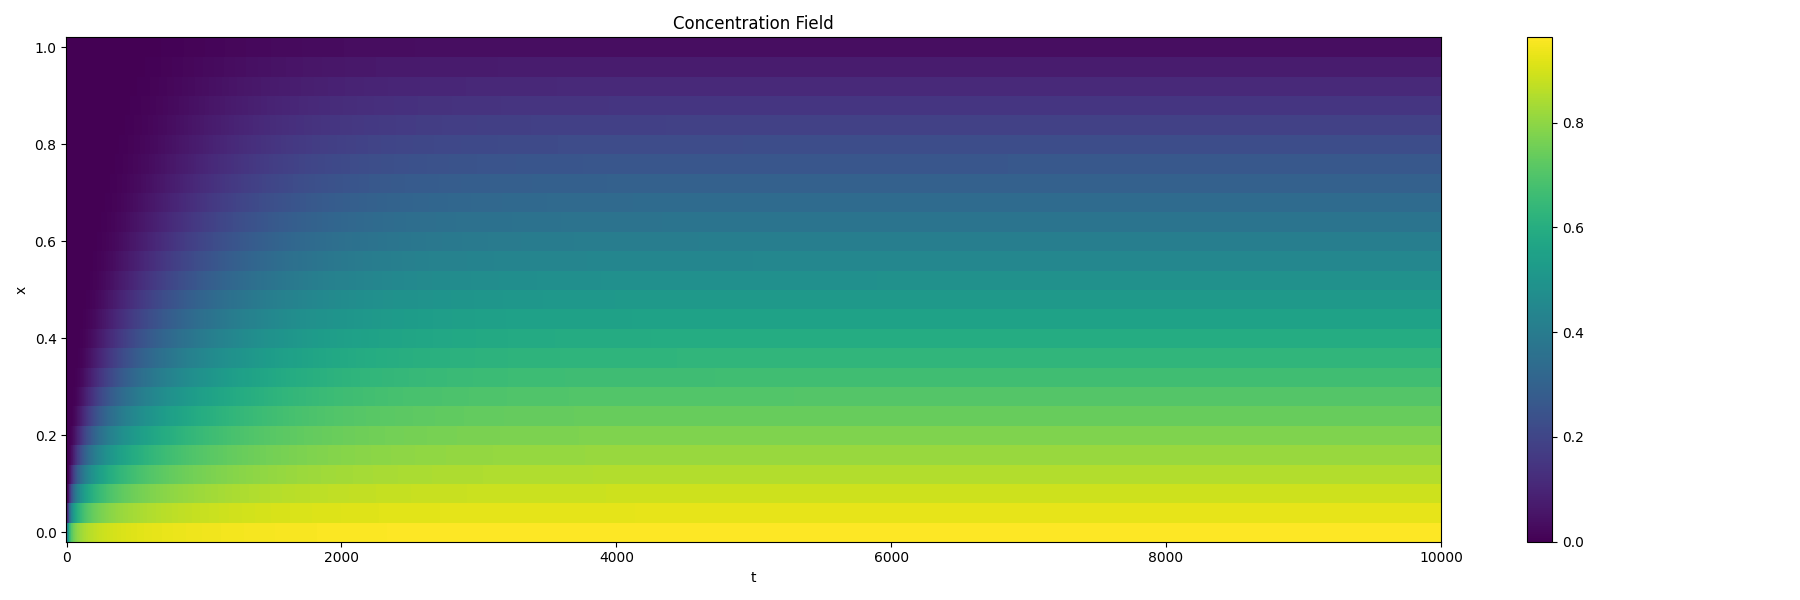
\includegraphics{figs/c_diss_field_full.png}
    \caption{Synthetic concentration field $c(x,t)$ generated using the Langmuir isotherm for a spatial domain of $x \in [0, 1]$ meters and a temporal domain of $t \in [0, 10000]$ days.}
    \label{fig:c_diss_field_full}
\end{figure}


The diffusion-sorption Equation ~\vref{eq:diff-sorpt-pde} reads:

\begin{equation}
    \frac{\partial c}{\partial t} = \frac{D}{R(c)} \frac{\partial^2 c}{\partial x^2},
    \label{eq:diff-sorpt-pde}
\end{equation}

where $c$ is the issolved contaminant concentration, $D$ represents the effective diffusion coefficient, $t$ is time, and $x$ is the distance along the flow path.

The following boundary conditions were considered here:

\begin{itemize}
    \item Top Boundary: At the top end of the sample where pure-phase TCE is injected, a Dirichlet boundary condition is used:

    \begin{equation}
        c|_{x=0} = c_{sol} \quad \forall t : 0 \leq t \leq T,
    \end{equation}

    where $c_{sol}$ is the solubility limit of TCE in water and $T$ is the experiment time.

    \item Bottom Boundary: At the bottom end of the sample, which is flushed with clean water, a Cauchy boundary condition is applied:

    \begin{equation}
        c|_{x=L} = \frac{D}{Q} \frac{\partial c}{\partial x} \quad \forall t : 0 \leq t \leq T,
    \end{equation}

    where $Q$ is the flow rate of the clean water and $L$ is the sample length.
\end{itemize}

The goal is to learn $\hat{R}(x,t;\theta)$ (represented by a neural network) given the data $\mathcal{D} = \{ (x_i, t_i, c_i) \}_{i=1}^N$ which consists of concentration measurements $c_i$ at spatial positions $x_i$ and temporal points $t_i$. The network needs to be trained such that the PDE solution using $\hat{R}$ minimizes the error with respect to the data.




\subsection{Finite Volume Neural Network (FINN)}

FINN is a specialized machine learning approach that combines the strengths of traditional numerical methods with the adaptability of neural networks to solve PDEs with unknown or uncertain components. It leverages the Finite Volume Method (FVM), dividing the problem domain into discrete control volumes. The core of FINN lies in its use of ``flux kernels'' $F_i$ – neural networks that learn how quantities flow between neighboring volumes. Specifically, each volume has a flux kernel composed of two subkernels, $f_{i-}$ and $f_{i+}$, one for each direction, which model these fluxes based on the concentrations in the volume and its neighbors. These subkernels consist of two parts: a ``stencil'' component $\Phi_N$ that approximates the FVM spatial scheme and a ``diffusivity'' component $\Phi_D$ that learns how the flow rate depends on the concentration itself:

\begin{align*}
    f_{i-} &= \Phi_D(c_i) \cdot \Phi_N(c_i, c_{i-1}) \\
    f_{i+} &= \Phi_D(c_i) \cdot \Phi_N(c_i, c_{i+1}).
\end{align*}

Furthermore, FINN employs ``state kernels'' $S_i$ that take the local concentration and calculated fluxes as input to update the concentration over time. This time evolution is governed by a Neural Ordinary Differential Equation (NODE) solver \cite{chen2019neuralordinarydifferentialequations}, a differentiable method that integrates seamlessly into the neural network training. By integrating FVM discretization, specialized neural network modules, and a NODE solver, FINN is capable of learning complex time-dependent spatial patterns while adhering to physical conservation laws and boundary conditions.



\subsection{Uniqueness of Inverse Problem}
\label{sec:uniqueness}

As a prerequisite for uncertainty quantification, it's crucial to investigate whether the inverse problem of determining the retardation factor, $R(c)$, from concentration data is unique. Non-uniqueness, meaning multiple possible $R(c)$ functions could produce the same concentration field, would complicate the interpretation of any UQ results. Instead of a purely theoretical analysis, we conduct an empirical investigation into the uniqueness of $R(c)$ for our specific problem.

Our approach leverages the available synthetic concentration data generated using known $R(c)$ functions (e.g., Langmuir, Freundlich, and linear isotherms). We rearrange the diffusion-sorption PDE (Equation \ref{eq:diff-sorpt-pde}) to explicitly solve for $R(c)$:

\begin{equation}
    R(c) = D \frac{\partial^2 c}{\partial x^2} \left/ \frac{\partial c}{\partial t} \right .
    \label{eq:rearranged_pde}
\end{equation}

We then numerically approximate the first-order time derivative ($\partial c / \partial t$) and the second-order spatial derivative ($\partial^2 c / \partial x^2$) of the concentration field $c(x,t)$ using a B-spline surrogate model. This spline allows us to estimate the derivatives at any point within the spatial and temporal domain of the data.

Figure \ref{fig:ret_uniqueness} shows the results of this empirical uniqueness analysis for three different synthetic datasets generated using the Langmuir, Freundlich, and linear isotherms. For each case, we plot the raw $R(c)$ estimates and the binned and averaged $R(c)$ values as a function of $c$. We also include a comparison with the analytical isotherms used to generate the synthetic datasets.

\begin{figure}[h]
    \centering
    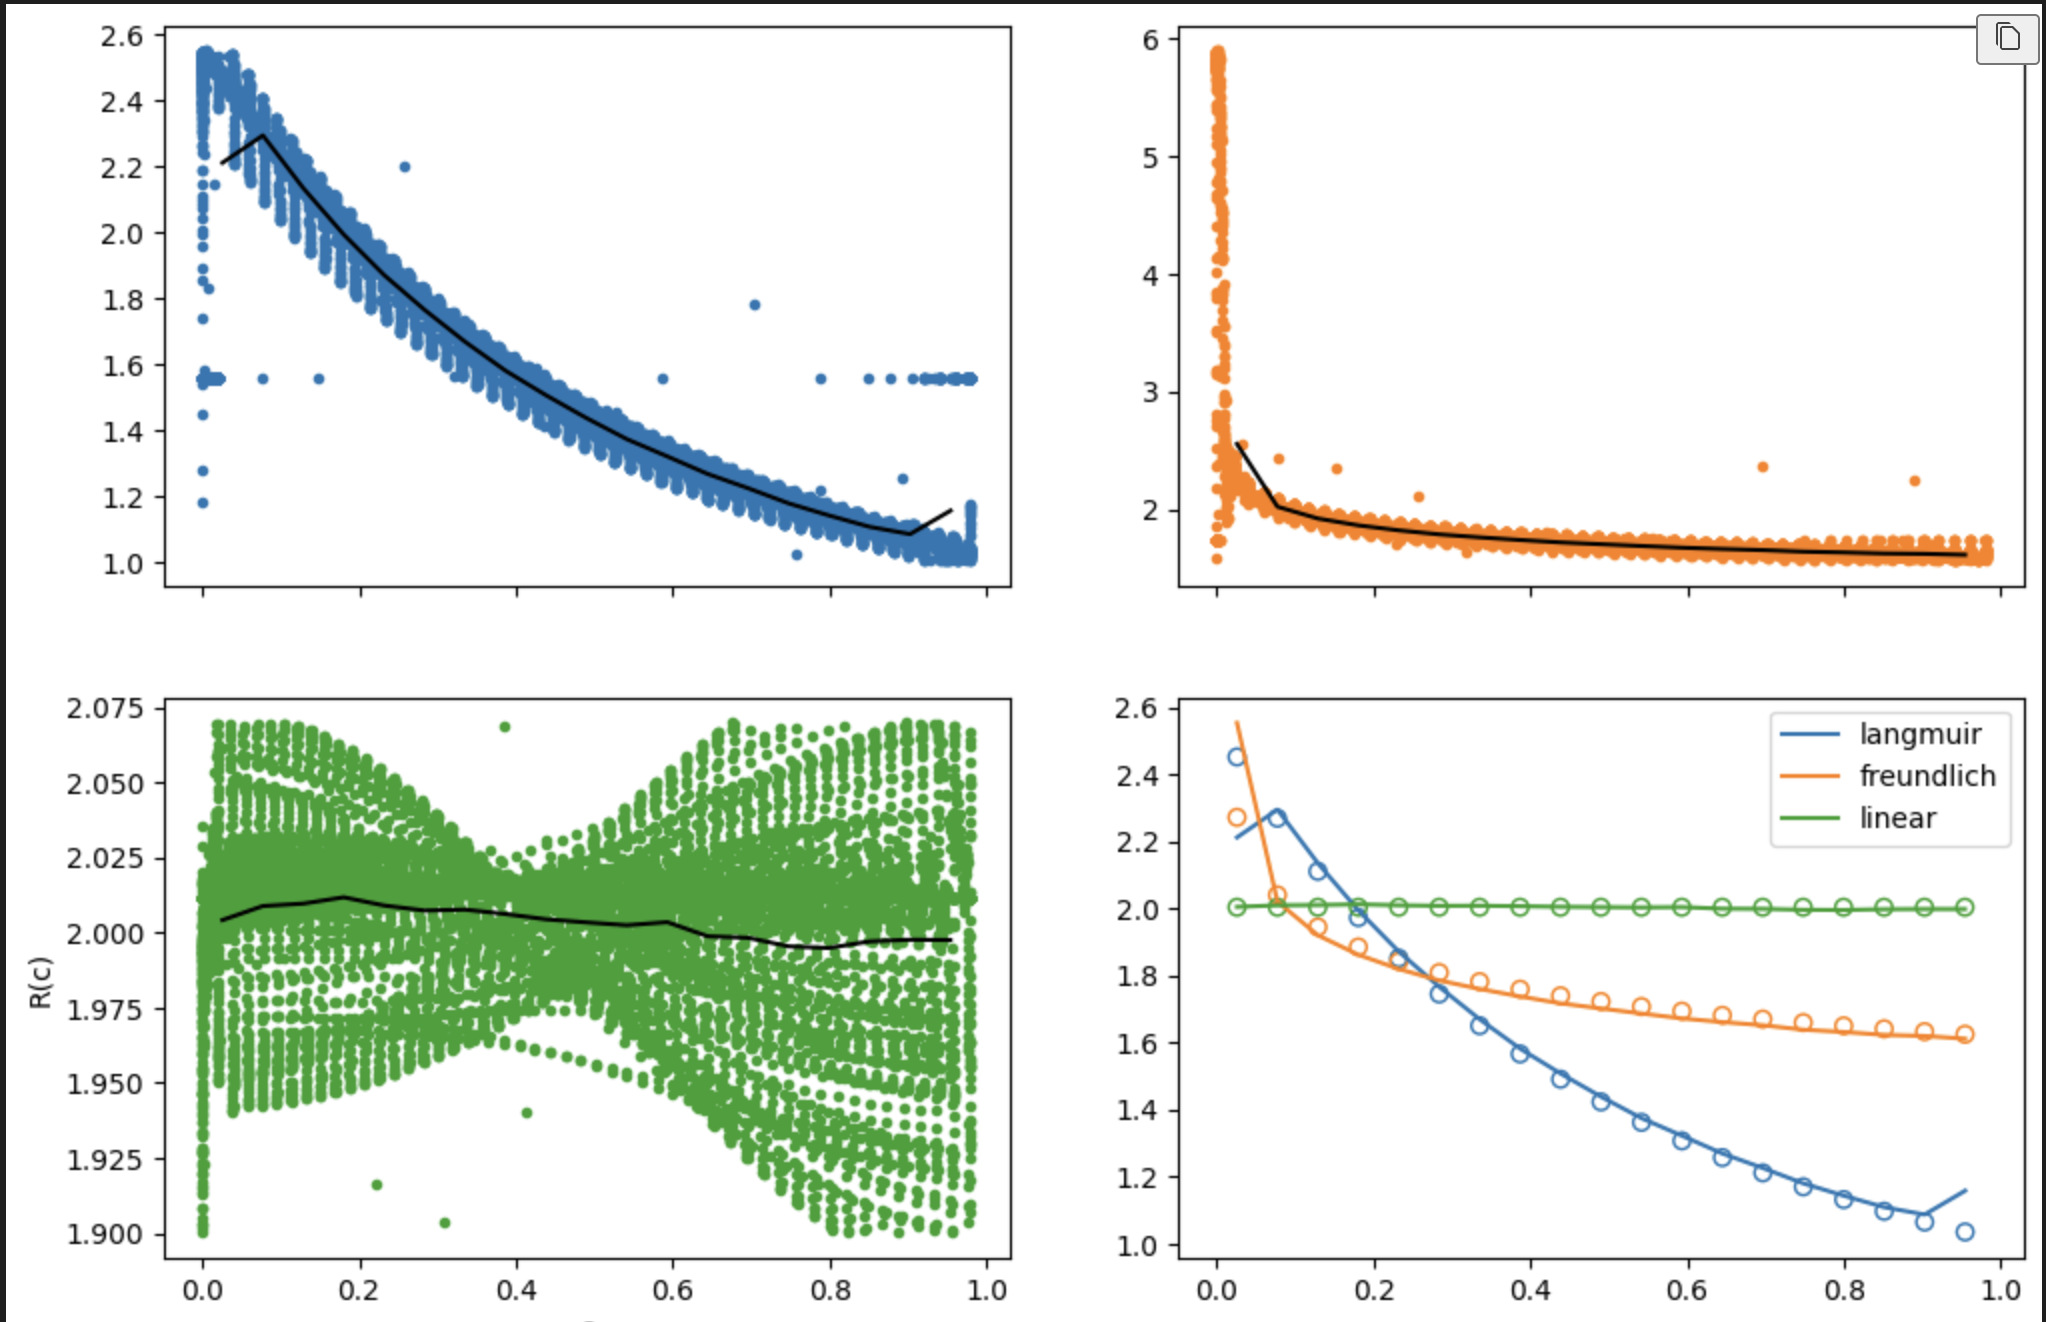
\includegraphics{figs/ret_uniqueness.png}
    \caption{Empirical investigation of the uniqueness of the retardation factor $R(c)$ for three different synthetic datasets generated using the Langmuir, Freundlich, and linear isotherms. The left and top panels show the raw $R(c)$ estimates (colored circles) and the binned and averaged $R(c)$ values (black line with circle markers) as a function of $c$. The bottom-right panel compares the binned and averaged $R(c)$ values (colored circle markers) with the analytical isotherms (colored line) used to generate the synthetic datasets. Error bars indicate the standard deviation inside the bin.}
    \label{fig:ret_uniqueness}
\end{figure}

The results suggest that, for these synthetic datasets, the inverse problem of determining $R(c)$ from concentration data is largely unique, apart from minor numerical inaccuracies. The binned and averaged $R(c)$ values closely follow the trend of the analytical isotherms, indicating that our approach can recover the underlying retardation behavior with reasonable accuracy.

This empirical evidence of uniqueness provides a foundation for subsequent uncertainty quantification. It suggests that discrepancies between different $R(c)$ solutions obtained using FINN can be attributed primarily to aleatoric uncertainty (e.g., measurement noise) and epistemic uncertainty (e.g., limitations in model knowledge) rather than inherent non-uniqueness in the inverse problem itself.
% TODO: Bad that I explain these uncertainties only in the next section?




\subsubsection{Uncertainty Quantification}
There are two main aspects of UQ in this context:
\begin{enumerate}
    \item UQ for FINN output: $p(\hat{c}(x,t) | \mathcal{D})$. This represents the probability distribution of the predicted contaminant concentration $\hat{c}(x,t)$ obtained from the FINN model, given the data $\mathcal{D}$.
    \item UQ for the predicted retardation factor: $p(\hat{R}(c) | \mathcal{D})$. This is arguably more important because it represents the probability distribution of the predicted retardation factor $\hat{R}(c)$ given the data $\mathcal{D}$. This distribution helps in understanding the confidence in the estimated retardation factor.
\end{enumerate}

But there are also two types of uncertainty that have to be differentiated \cite{depeweg2018decomposition, gawlikowski2023survey}:

\begin{enumerate}
    \item Aleatoric uncertainty: This arises from inherent randomness in the data and the physical system. It is irreducible and is caused by factors such as measurement noise and variability in the system parameters.
    \item Epistemic uncertainty: This stems from limited knowledge of the model (e.g. uncertainty over its parameters). It is associated with model structure, neural network architecture, and limited training data. It quantifies the model's predictive uncertainty.
\end{enumerate}

While a clear decomposition into aleatoric and epistemic uncertainty is often challenging, as seen with methods like BNNs using MCMC, our primary focus is on quantifying the overall predictive uncertainty, which includes both components. However, our method has the added advantage of decomposing the uncertainty by design, providing a more precise and interpretable quantification of both aleatoric and epistemic uncertainties.





\subsection{Bayes Neural Networks}
\label{sec:bayes_nn}
% TODO: Maybe too detailed. Move some to appendix?
This section describes the baseline methodology used for comparison, which employs Bayesian Neural Networks and MCMC to estimate the posterior distribution of the retardation factor, $\hat{R}(c(x,t))$, parameterized by a neural network (NN). The retardation factor is a function of concentration, $c$, which itself is a function of spatial position, $x$, and time, $t$. This approach updates prior beliefs about the retardation factor based on observed data, $\mathcal{D}$.

\paragraph{Prior Distribution:}

A Gaussian prior distribution, $p(\theta)$, is placed over the NN parameters $\theta$, reflecting prior knowledge or assumptions. This prior is centered on the parameters $\theta_{PT}$ of a pre-trained NN, with covariance matrix $\Sigma_p = 0.05 \, I$:


\begin{equation*}
p(\theta) = \mathcal{N}(\theta | \theta_{PT}, \Sigma_p)
\end{equation*}

\paragraph{Likelihood Function:}

The likelihood function, $p(\mathcal{D} | \theta)$, quantifies the probability of observing the data $\mathcal{D}$ given a specific set of NN parameters $\theta$. We assume additive Gaussian noise with standard deviation $\sigma$ corrupts the observed concentrations. Let $c_{obs}(x,t)$ represent the observed concentration at position $x$ and time $t$, and $c_{model}(x,t; \theta)$ the concentration predicted by the model (using a FINN solver with $\hat{R}(c(x,t);\theta)$). The likelihood is:

\begin{equation}
p(\mathcal{D} | \theta) = \prod_{(x_i, t_i, c_i) \in \mathcal{D}} \frac{1}{\sqrt{2\pi \sigma^2}} \exp \left( -\frac{(c_i - c_{model}(x_i, t_i; \theta))^2}{2\sigma^2} \right)
\label{eq:likelihood}
\end{equation}

\paragraph{Posterior Distribution:}

Bayes' theorem provides the posterior distribution of the NN parameters given the data:

% TODO: is this good notation?
\begin{equation*}
p(\theta | \mathcal{D}) \propto p(\mathcal{D} | \theta) p(\theta)
\end{equation*}

\cite{finn} compare several methods to obtain samples from this distribution, including the Metropolis-Hastings algorithm, the MALA algorithm, and the Barker method. The accepted samples $\{\theta_i\}$ from the used algorithm are then treated as draws from the posterior distribution $p(\theta | \mathcal{D})$.

\paragraph{Posterior of Retardation Function:}

Finally, the posterior distribution of the retardation factor $\hat{R}(c)$ is obtained by evaluating the NN with the sampled parameters $\{\theta_i\}$:

\begin{equation*}
\{\hat{R}(c | \theta_i)\} \sim p(\hat{R}(c) | \mathcal{D})
\end{equation*}

This set of retardation factor samples provides a probabilistic description of the retardation behavior, incorporating the uncertainty arising from the limited and noisy data.

Since \cite{finn} obtain the best results with the Barker method and no burn-in period by starting from the pre-trained model, we follow their approach to have a fair comparison.




\subsection{PI3NN (Prediction Intervals from Three Neural Networks)}
PI3NN \cite{pi3nn} is a method for constructing prediction intervals (PIs) that uses three independently trained neural networks. It aims to provide tight, non-crossing PIs across various confidence levels without requiring retraining for each level.

The method's theoretical foundation lies in approximating the ground-truth PI bounds with a family of neural networks. Specifically, PI3NN approximates the median of the target variable, $M[y]$, and the expected deviations above and below the median, $E[(y - M[y]) \ind{y-M[y]>0}]$ and $E[(M[y] - y) \ind{M[y]-y>0}]$, respectively, using three independently trained neural networks ($f_w(x)$, $u_\theta(x)$, and $l_\epsilon(x)$). These networks are trained using the standard mean squared error loss, simplifying the training process and avoiding the need for specialized loss functions and sensitive hyperparameters that often require fine-tuning in other PI methods.

Once trained, PI3NN constructs the PI bounds as linear combinations of the three networks' outputs. The coefficients of these linear combinations ($\alpha$ and $\beta$) are determined through a root-finding algorithm that ensures the desired PICP (Prediction Interval Coverage Probability) for a given confidence level $q$ ($\gamma$ in \cite{pi3nn}). This process allows for calculating PIs for multiple confidence levels without retraining the networks, offering significant computational advantages.


Figure ~\vref{fig:3pinn_illustration} illustrates the 6-step breakdown of the PI3NN process:
\begin{enumerate}
    \item \textbf{Learn the mean:} Train a neural network to approximate the mean of the target data.
    \item \textbf{Estimate the median:} Calculate the median by shifting the learned mean.
    \item \textbf{Calculate and split residuals:} Compute the residuals between the actual data and the estimated median, then separate these into positive and negative residuals.
    \item \textbf{Learn residuals:} Train two more neural networks, one to approximate the positive residuals and the other to approximate the negative residuals.
    \item \textbf{Construct PI:} Calculate a PI using the learned median and the learned positive and negative residuals.
    \item \textbf{Generate multiple PIs:} Use a root-finding algorithm to compute PIs for different confidence levels $q$ without retraining the networks.
\end{enumerate}


\begin{figure}[h]
    \centering
    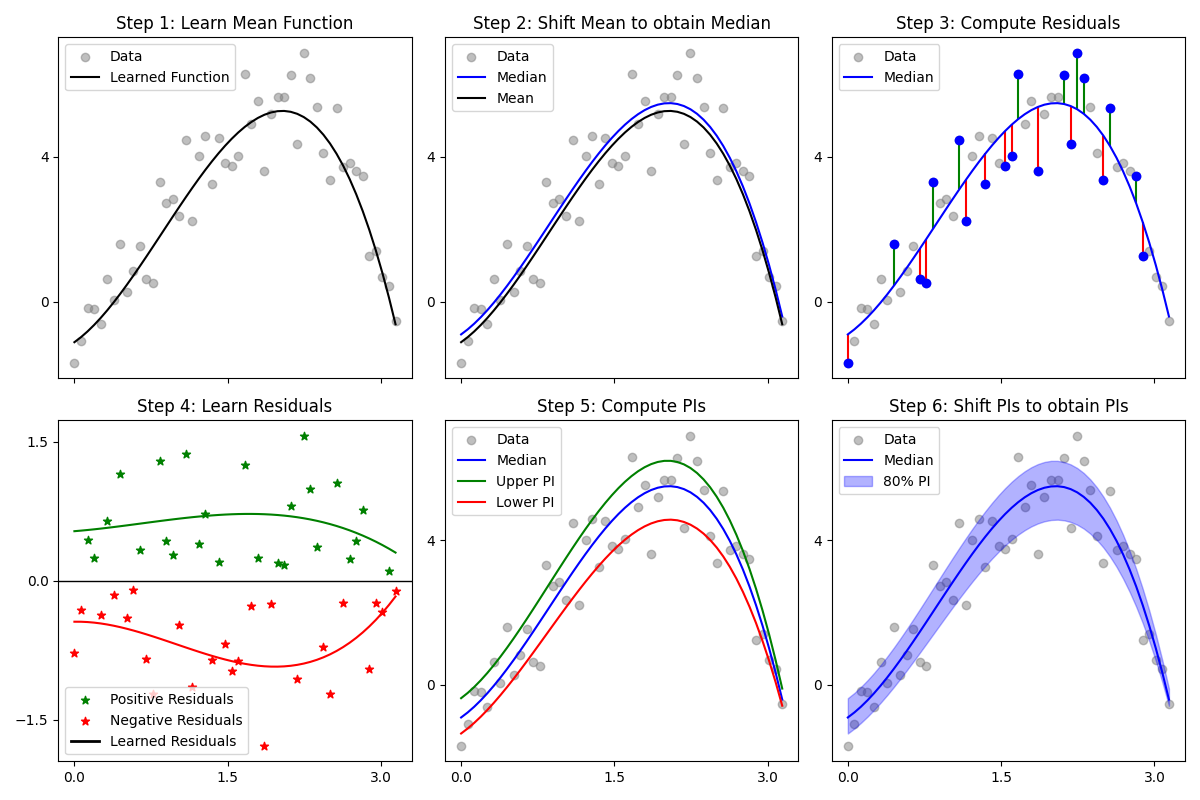
\includegraphics{figs/3pinn_illustration.png}
    \caption{Illustration of the PI3NN method.}
    \label{fig:3pinn_illustration}
\end{figure}





\section{Methodology}
\subsection{SPAN (Stochastic Perturbation Analysis of Networks)}
% SPAN = Epistemic uncertainty
Our objective is to determine the posterior predictive distribution $p(\hat{R}(c; \theta) = R(c)| \mathcal{D})$, which represents the probability of computing a specific retardation factor value $R(c)$ for a given concentration $c$, based on the observed breakthrough curve data $\mathcal{D}$. We present a method that computes this distribution by marginalizing over uncertain factors, denoted by $\mathcal{X}$, of the model and employing an approximate likelihood function $p(\mathcal{D} | \mathcal{X})$ based on the same assumtion of a normally disturbed dataset that was used for the Bayes approach.

\subsubsection{Approximating the Posterior Predictive Distribution via Marginalization over Uncertain Factors}

\paragraph{Model Formulation:}

We represent our neural network as $\hat{R}(c; \theta)$, where $c$ is the input concentration and $\theta$ denotes the network's parameters (weights and biases). The parameters $\theta$ are determined by a deterministic solver $S(\mathcal{X}, \mathcal{D})$, which takes hyperparameters $h$ and training data $\mathcal{D}$ as input. A prior distribution $p(h)$ is assigned over the hyperparameters; the exact form of $p(h)$ is not crucial, as it suffices to generate samples from it.

With $w(h) = \frac{p(\mathcal{D} | h)}{p(\mathcal{D})}$, the posterior predictive distribution can be expressed as:

\begin{align*}
p(\hat{R}(c; \theta) = R(c)| \mathcal{D}) &= \int p(\hat{R}(c; \theta) | h, \mathcal{D})\; p(h | \mathcal{D}) \, dh \\
                                          &= \int p(\hat{R}(c; \theta) | h, \mathcal{D})\; \frac{p(\mathcal{D} | h) p(h)}{p(\mathcal{D})} \, dh \\
                                          &= \int p(\hat{R}(c; \theta) | h, \mathcal{D})\; w(h)\; p(h) \, dh \\
                                          &= \int \delta(\hat{R}(c; \theta) - R(c))\; w(h)\; p(h) \, dh \\
\end{align*}

The first step is the marginalization over $h$, the second the application of Bayes' Theorem, and the last stems from the fact that the solver $\theta = S(h, \mathcal{D})$ is deterministic given $h$ and $\mathcal{D}$ and thus the distribution becomes a delta distribution.


\paragraph{Importance Sampling:}

So sampling from $p(\hat{R}(c; \theta) = R| \mathcal{D})$ becomes equivalent to sampling from $p(h)$, evaluating the solver to obtain the model parameters $\theta = S(h, \mathcal{D})$, evaluating the model $\hat{R}(c; \theta)$, and reweighting the samples with $w(h)$. This is the concept of importance sampling. To approximate the distribution, we thus have to draw $M$ samples $\{h_m\}_{m=1}^M$ from the prior distribution $p(h)$ and calculate the importance weight for each:

\begin{equation*}
w_m = \frac{p(\mathcal{D} | h_m)}{p(\mathcal{D})} \propto p(\mathcal{D} | h_m)
\end{equation*}

As $p(\mathcal{D})$ is a constant, it can be omitted, and the weights can be normalized subsequently.


\paragraph{Likelihood Computation:}
We use the same assumption about our data that the Bayesian baseline uses which results in an easy computation of the likelihood by just substituting $\theta$ with $S(h, \mathcal{D})$ in Equation ~\vref{eq:likelihood}:

\begin{equation*}
p(\mathcal{D} | h) = \prod_{x_i, t_i, c_i \in \mathcal{D}} \frac{1}{\sqrt{2\pi \sigma^2}} \exp \left( -\frac{(c_i - c_{model}(x_i, t_i; S(h, \mathcal{D})))^2}{2\sigma^2} \right)
\end{equation*}



\subsubsection{Data-SPAN}
% TODO: Data-SPAN = Aleatoric uncertainty
The exact same derivation can be applied when we assume a random dataset $\tilde{\mathcal{D}}$ instead of random hyperparameters $h$:

\begin{align*}
    p(\hat{R}(c; \theta) = R(c)| \mathcal{D}) &= \int p(\hat{R}(c; \theta) | \tilde{\mathcal{D}}, \mathcal{D})\; p(\tilde{\mathcal{D}} | \mathcal{D}) \, d \tilde{\mathcal{D}} \\
                                              &= \int p(\hat{R}(c; \theta) | \tilde{\mathcal{D}}, \mathcal{D})\; \frac{p(\mathcal{D} | \tilde{\mathcal{D}}) p(\tilde{\mathcal{D}})}{p(\mathcal{D})} \, d \tilde{\mathcal{D}} \\
                                              &= \int p(\hat{R}(c; \theta) | \tilde{\mathcal{D}}, \mathcal{D})\; w(\tilde{\mathcal{D}})\; p(\tilde{\mathcal{D}}) \, d \tilde{\mathcal{D}} \\
                                              &= \int \delta(\hat{R}(c; \theta) - R(c))\; w(\tilde{\mathcal{D}})\; p(\tilde{\mathcal{D}}) \, d \tilde{\mathcal{D}} \\
\end{align*}

\begin{equation*}
    p(\mathcal{D} | \tilde{\mathcal{D}}) = \prod_{x_i, t_i, c_i \in \mathcal{D}} \frac{1}{\sqrt{2\pi \sigma^2}} \exp \left( -\frac{(c_i - c_{model}(x_i, t_i; S(h, \tilde{\mathcal{D}})))^2}{2\sigma^2} \right)
\end{equation*}

\paragraph{Random Dataset Sampling:}
\label{sec:random_dataset_sampling}
To generate random datasets, we leverage PI3NN, applying it to the original breakthrough curve (BTC) dataset $\mathcal{D}$. Let $\hat{c}(t; \theta_{\mathcal{D}})$ be the mean concentration curve predicted by FINN trained on the full dataset $\mathcal{D}$, with $\theta_{\mathcal{D}}$ representing the learned FINN parameters. This FINN-predicted mean curve is used as input to the PI3NN algorithm, as it provides a more accurate representation of the underlying process compared to the mean curve learned by a standard MLP within the PI3NN framework.

PI3NN then learns the residuals, effectively modeling the distribution of $c$ given $t$. Let $F^{-1}(q | t)$ denote the quantile function predicted by PI3NN, where $q \in [0, 1]$ is the quantile level and $t$ is the time point. This function provides the concentration value at time $t$ corresponding to the $q$-th quantile of the learned distribution (see Figure ~\vref{fig:btc_dataspan_quantiles}).

To create a random dataset sample $\tilde{\mathcal{D}}(q)$, we sample a quantile level $q$ from a uniform distribution $\mathcal{U}(0, 1)$. Then, the random dataset sample is constructed as:

$$
\tilde{\mathcal{D}}(q) = \{ (t_i, F^{-1}(q | t_i) ) \}_{i=1}^N
$$

This process is repeated $M$ times to obtain a collection of random datasets $\{\tilde{\mathcal{D}}_j\}_{j=1}^M$. Each $\tilde{\mathcal{D}}_j$ is then used to train a separate instance of FINN, effectively providing a set of retardation factor samples, analogous to the samples obtained from the hyperparameter perturbation approach.

To enhance the accuracy of the likelihood computation in Section \vref{sec:likelihood}, we intentionally include the quantile levels $0$ and $1$ in the random samples. This improves the fit of the distribution to the histogram of the samples.

\begin{figure}[h]
    \centering
    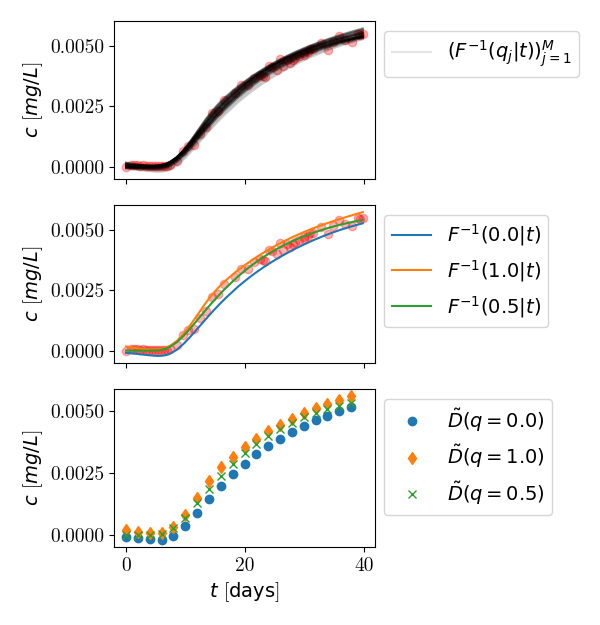
\includegraphics{figs/btc_dataspan_quantiles.png}
    \caption{Left: BTC quantile functions for all quantile samples $q_j$. Middle: BTC quantile functions for quantiles $0$, $0.5$, and $1$. Right: BTC datasets for quantiles $0$, $0.5$, and $1$.}
    \label{fig:btc_dataspan_quantiles}
\end{figure}



\section{Data and Setup}

\subsection{Experimental Setup}
The experiments were conducted using Python 3.11.3. Modified versions of the FINN code from \cite{finn} and the PI3NN code from \cite{pi3nn} were used. The code and specific library versions are available on GitHub. GNU parallel \cite{tange_2023_10199085} was used for parallel execution of experiments. % TODO: insert github link

\subsection{Data Acquisition}
The BTC data was obtained from the work by \cite{finn}, originally sourced from \cite{nowak2016entropy}. Synthetic data was generated using the same solver employed by FINN, ensuring consistency in the experimental setup.

\subsection{Training Details}
Early stopping was implemented to halt training when the loss plateaued. Training runs for FINN were discarded if the normalized mean squared error (NMSE) exceeded $10^{-5}$ (measured on BTC), ensuring a minimum level of accuracy in the learned retardation factor.

\begin{equation*}
    \text{NMSE}(y, \hat{y}) = \text{MSE}(y, \hat{y}) / \text{mean}(y)
\end{equation*}




\section{Experiments}

\subsection{SPAN}
The hyperparameters that were used differ for the synthetic data case and the experimental data case:

\begin{table}[h!]
    \centering
    \begin{tabular}{>{\raggedleft\arraybackslash}m{3.5cm} | >{\raggedright\arraybackslash}m{3cm} >{\centering\arraybackslash}m{2.5cm} >{\centering\arraybackslash}m{2.5cm}}
        \toprule
        \textbf{Hyperparameter} & \textbf{Description} & \textbf{Experimental} & \textbf{Synthetic} \\
        \midrule
        Weight Initialization & \small{Seed for initial values for model weights} & \textcolor{green}{\checkmark} & \textcolor{green}{\checkmark} \\
        \midrule
        Training Data Mask (see Figure ~\vref{fig:training_data_mask}) & \small{Seed for mask applied to training data} & \textcolor{red}{\ding{55}} & \textcolor{green}{\checkmark} \\
        \midrule
        Training Data Noise & \small{Seed for noise added to training data} & \textcolor{red}{\ding{55}} & \textcolor{green}{\checkmark} \\
        \midrule
        Max Epochs & \small{Maximum number of training iterations} & \textcolor{green}{\checkmark} & \textcolor{red}{\ding{55}} \\
        \midrule
        MSE Loss Factor & \small{Factor for Mean Squared Error loss} & \textcolor{green}{\checkmark} & \textcolor{red}{\ding{55}} \\
        \midrule
        Physical Loss Factor & \small{Factor for physical loss} & \textcolor{green}{\checkmark} & \textcolor{red}{\ding{55}} \\
        \bottomrule
    \end{tabular}
    \caption{Hyperparameters for Experimental and Synthetic Settings}
    \label{tab:hparams}
\end{table}

In the experimental setting, $780$ samples were generated using the specified hyperparameters. For the synthetic experiments, the number of samples varied and is indicated in the respective figure captions for clarity and comparison within those specific contexts. The experimental results are shown in Figure ~\vref{fig:span_samples}.
% TODO: synthetic results

\begin{figure}[h]
    \centering
    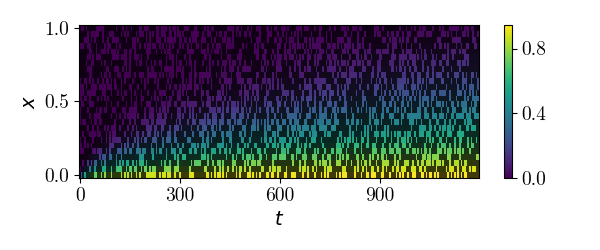
\includegraphics{figs/c_diss_field_train_random_subset.png}
    \caption{Full synthetic concentration training data where 50\% of datapoints are randomly masked (dark patches).}
    \label{fig:training_data_mask}
\end{figure}


\subsection{Data-SPAN}
This approach was applied only to the experimental data because the synthetic training data lacks noise, leading to extremely small residuals and a very narrow distribution that does not impact sampling.

For the experimental data, we sampled $70$ quantiles as detailed in Section ~\vref{sec:random_dataset_sampling}. The results are shown in Figure ~\vref{fig:dataspan_samples}.



\subsection{Full-SPAN}
This approach is equivalent to Data-SPAN but additionally, for every sampled quantile, the hyperparameters are also randomly sampled. The results are shown in Figure ~\vref{fig:fullspan_samples}.


\subsection{Baselines (Bayes NN via MCMC)}
We computed $10$k samples using the same parameters as \cite{finn}; the samples are visualized in Figure ~\vref{fig:mcmc_samples}.
% TODO: Why 10k? This is very important to know for arguing about efficiency.

% This is not a result (of me) thus it is here and not in the results section
\begin{figure}[h]
    \centering
    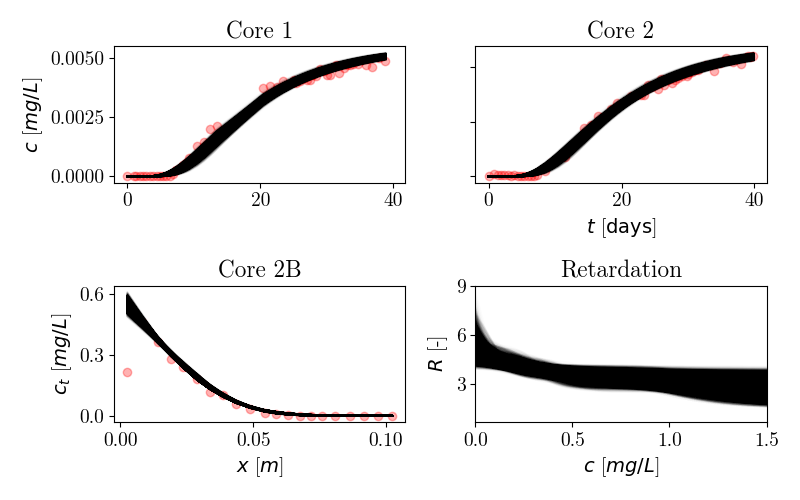
\includegraphics{figs/finn_mcmc_samples.png}
    \caption{Retardation curves generated by MCMC sampling as detailed in Section ~\vref{sec:bayes_nn}.}
    \label{fig:mcmc_samples}
\end{figure}





\section{Results}
\subsection{Samples and Prediction Intervals}
\subsubsection{Synthetic Data}

\paragraph{SPAN}
When the hyperparameters are randomly sampled to learn different retardations, the uncertainty in $R(c)$ is very small as can be seen in Figure ~\vref{fig:synthetic_SPAN_factors_PIs}, even when all hyperparameters are combined in ``All UQ''.

% TODO: Get rid of upper right triangle
\begin{figure}[h]
    \centering
    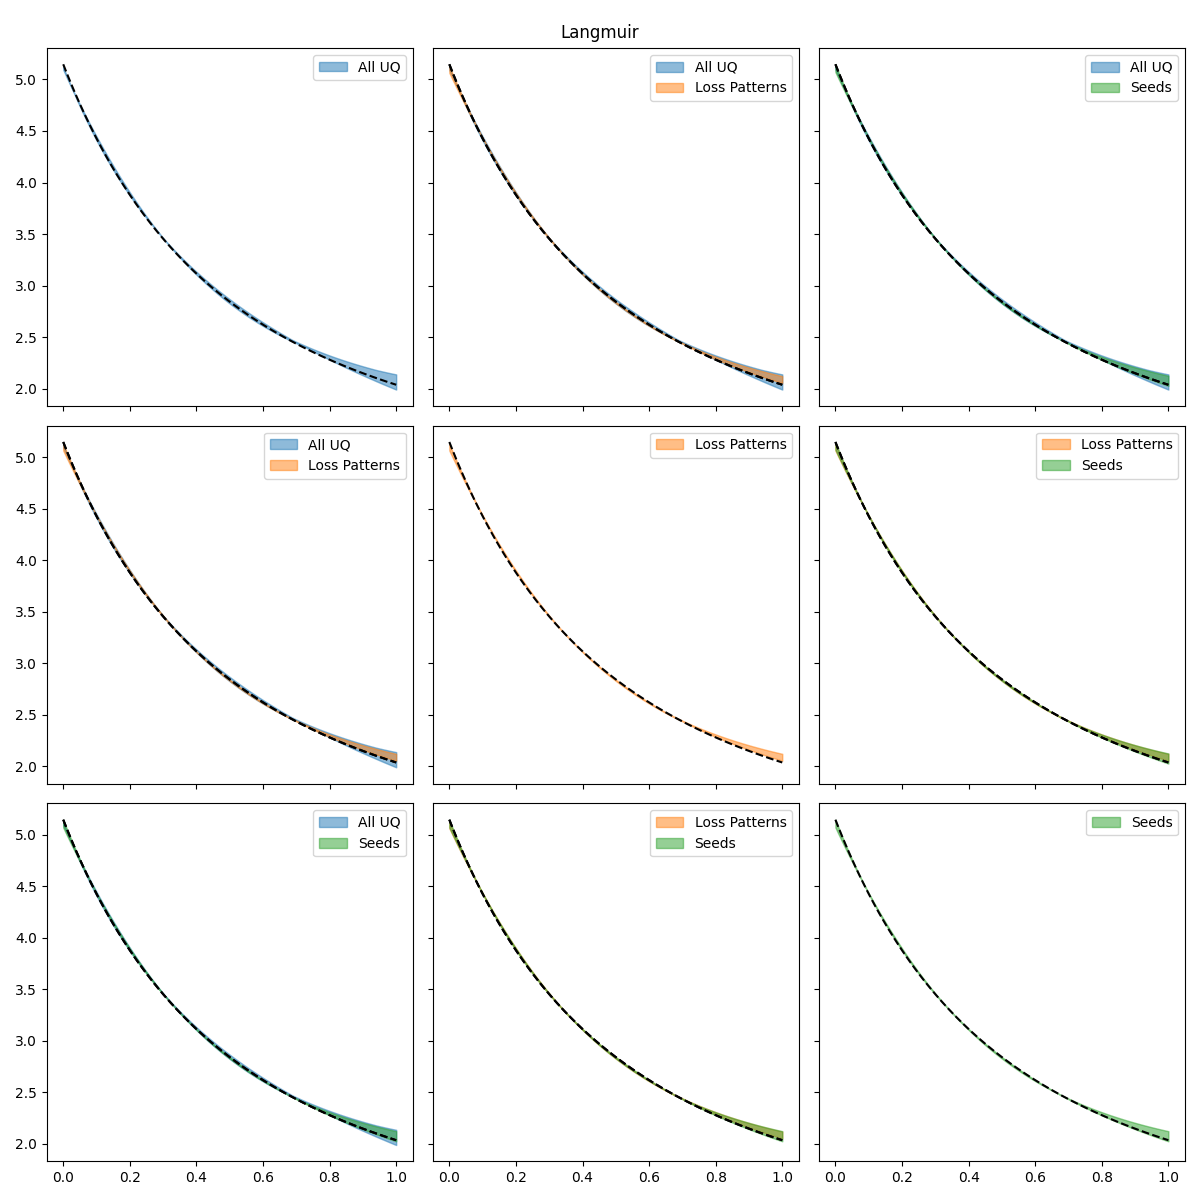
\includegraphics{figs/finn_synthetic_SPAN_factors_PIs.png}
    \caption{Comparison of retardation PIs obtained via SPAN on synthetic data (generated by langmuir isotherm).}
    \label{fig:synthetic_SPAN_factors_PIs}
\end{figure}

\paragraph{Data-SPAN}
When applying gaussian noise of the same strength as the experimental data has due to measurement error \cite{nowak2016entropy}, the uncertainty in $R(c)$ becomes much larger compared to SPAN as can be seen in Figure ~\vref{fig:synthetic_langmuir_c_noise}.

\begin{figure}[h]
    \centering
    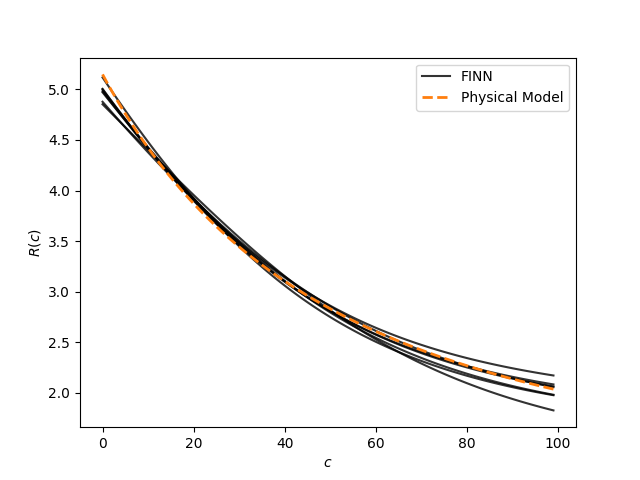
\includegraphics{figs/finn_synthetic_langmuir_c_noise.png}
    \caption{Retardations learned by FINN on synthetic dataset (generated by langmuir isotherm) pertubed by gaussian noise.}
    \label{fig:synthetic_langmuir_c_noise}
\end{figure}



\subsubsection{Experimental Data}

Figure ~\vref{fig:mcmc_vs_fullspan} illustrates that the 90\% PIs for both the MCMC and full SPAN methods encompass similar concentration values. This agreement arises from their comparable coverage of $R(c)$ values when $c \leq 1$. While the methods diverge for larger values of $c$, this discrepancy has minimal impact on the concentration fields, as these are less sensitive to $R(c)$ in that regime. Given that full SPAN produces similar $c$ PIs but incorporates larger uncertainty in $R$, it provides a more robust uncertainty estimate. A more quantitative exploration of these findings is presented in the following sections.


\begin{figure}[h]
    \centering
    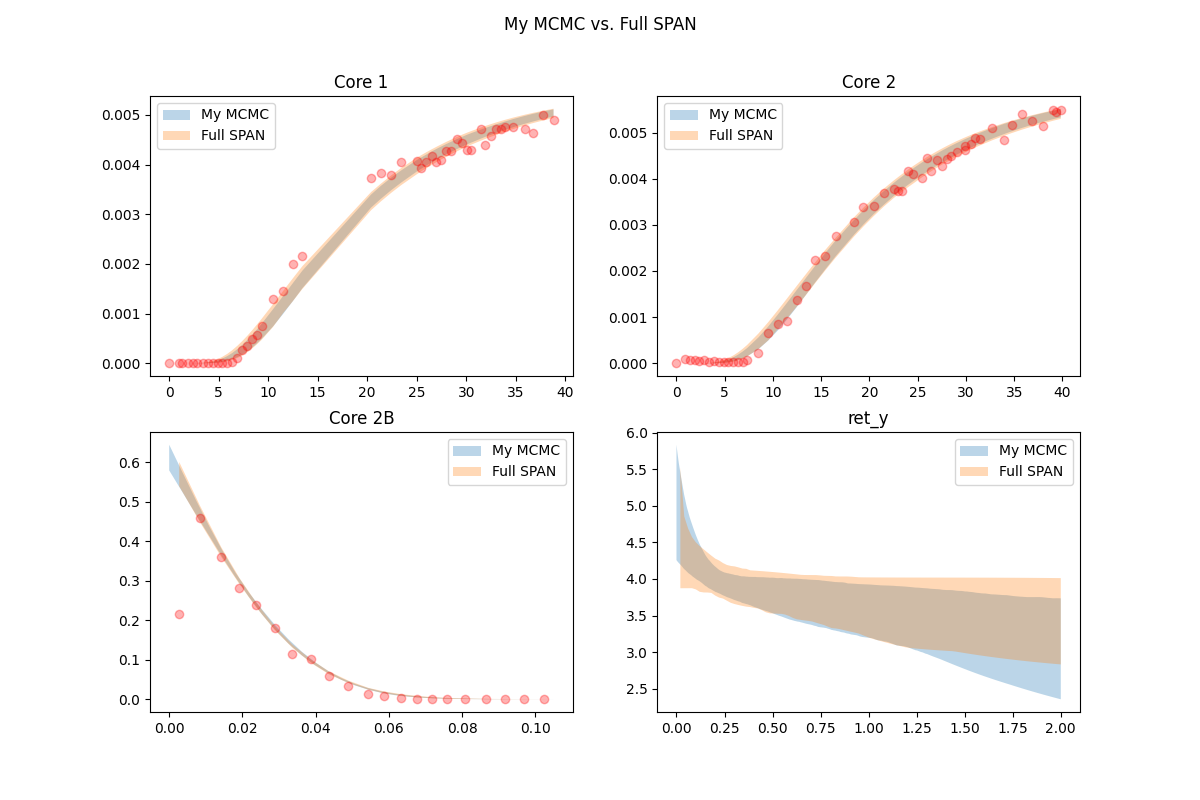
\includegraphics{figs/finn_My MCMCvsFull SPAN_PIs.png}
    \caption{Retardation PIs and correspoding concentration PIs obtained from it by training FINN with random hyperparameters and random datasets using PI3NN (orange). Compared with MCMC approach (blue). (90\% PIs are depicted.)}
    \label{fig:mcmc_vs_fullspan}
\end{figure}


\begin{figure}[h]
    \centering
    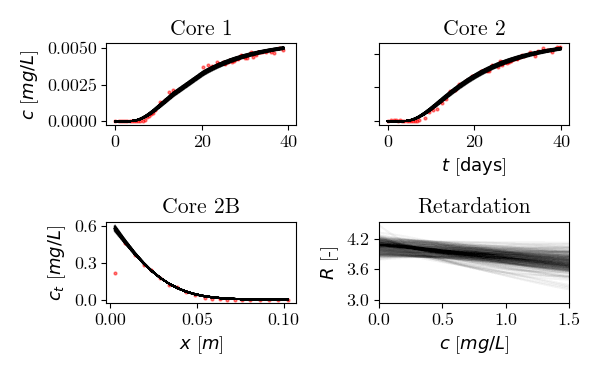
\includegraphics{figs/finn_span_samples.png}
    \caption{Retardation samples and correspoding concentration curves obtained from it by training FINN with random hyperparameters.}
    \label{fig:span_samples}
\end{figure}

\begin{figure}[h]
    \centering
    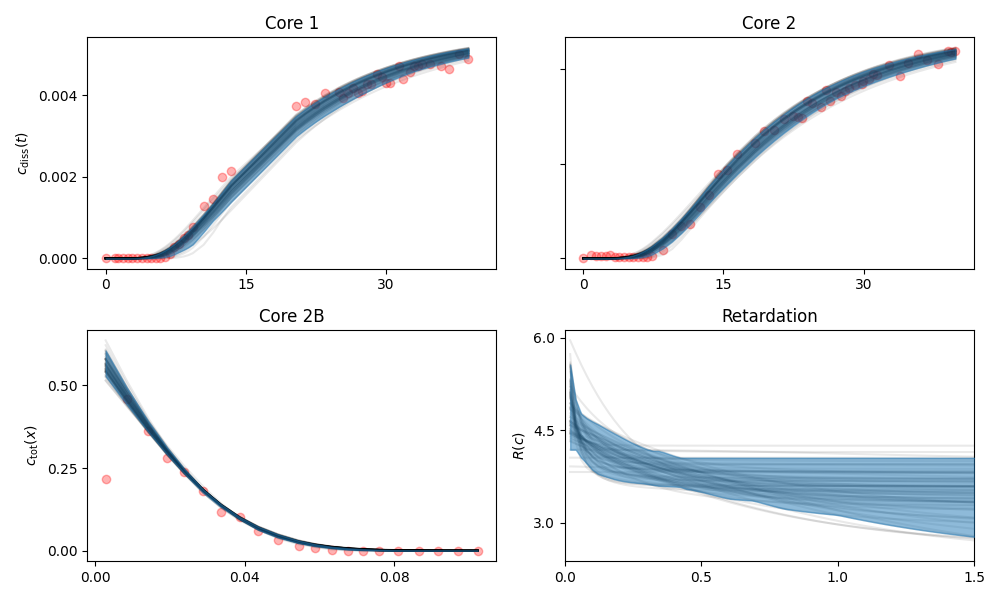
\includegraphics{figs/finn_dataspan_samples.png}
    \caption{Retardation samples and correspoding concentration curves obtained from it by training FINN with random datasets using PI3NN.}
    \label{fig:dataspan_samples}
\end{figure}

% TODO: Simulations for this have not been done yet.
\begin{figure}[h]
    \centering
    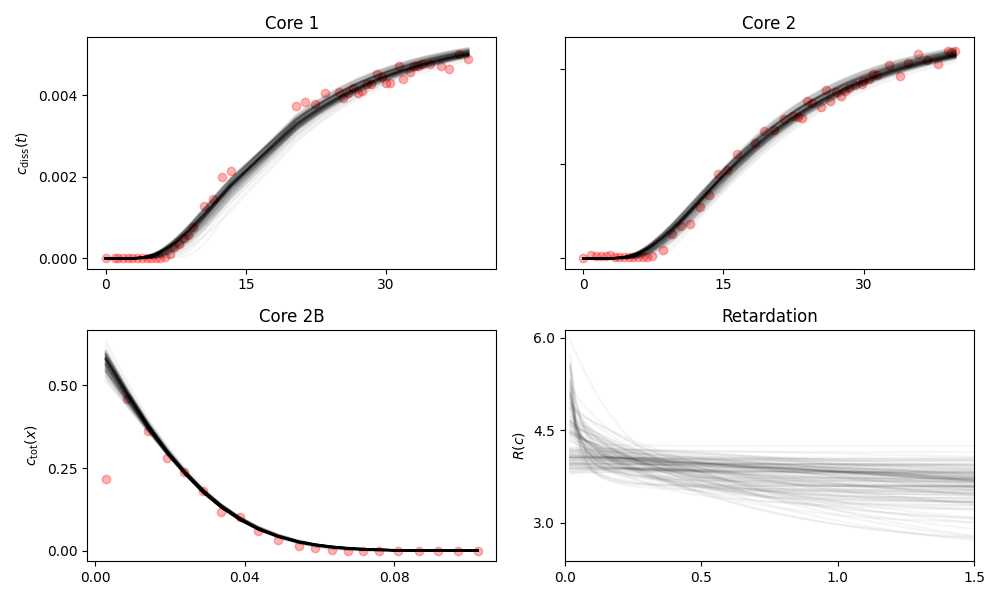
\includegraphics{figs/finn_fullspan_samples.png}
    \caption{Retardation samples and correspoding concentration curves obtained from it by training FINN with random hyperparameters and random datasets using PI3NN.}
    \label{fig:fullspan_samples}
\end{figure}




\subsection{Runtime}
We measure and compare the runtime of generating a single sample of our method and the baseline. Since SPAN as well as Data-SPAN require training of the NN from scratch for each sample, the runtime approximately equals the training time. Averaging over $10$ trials, the runtime is $170$ seconds.

The MCMC method uses thinning, saving only every $10$th sample. The average runtime for this is about $11.4$ seconds, almost $15$ times faster than our method.
% TODO: But how many samples does each method need?
% TODO: And what if the log posterior trace plot is still decreasing? Am I even allowed to take samples from it then?
% TODO: What about parallelization? Our method is trivially paralellizable. What about MCMC with Barker sampler?
% TODO: What about other problems (with e.g. more weights). Does our method get better then?



% Bit unnecessary plot?
\begin{figure}[h]
    \centering
    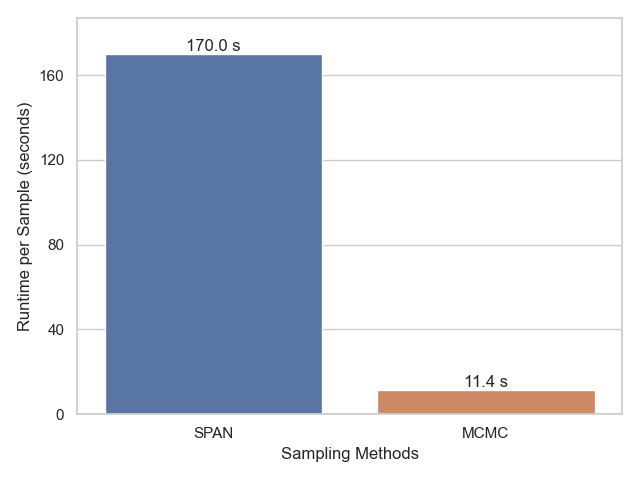
\includegraphics{figs/runtime_per_sample.png}
    \caption{Runtime for generating a single sample using SPAN (left bar) and MCMC (right bar). Measured on the same machine and averaged over $10$ trials. Variance is too insignificant to matter here.}
    \label{fig:runtime_per_sample}
\end{figure}

\subsection{Likelihood}
\label{sec:likelihood}
To evaluate the predictive quality of our method, we use its samples to estimate a probability distribution. This is done by computing a histogram. We can then estimate the likelihood of the training data $\mathcal{D}$ given this distribution. We transform the likelihood into a negative log-likelihood (NLL) to obtain more accurate results. A lower NLL is better. Applying this procedure on SPAN yields a NLL of $-6.41$, $-7.11$ for MCMC, and $-7.14$ for Data-SPAN. A good baseline to compare this against, is a normal distribution around the FINN BTC prediction mean and standard deviation equal to the sample standard deviation computed from the residuals:
\begin{equation*}
    p(c; t) = \frac{1}{\sqrt{2 \pi \mathcal{s}^2}} \exp(-\frac{1}{2 \mathcal{s}^2} (\hat{c}(x=L, t; \theta_{\mathcal{D}}) - c)^2)
\end{equation*}
This yields a NLL of $-7.50$, which is the lowest value. % TODO: Interpretation

\subsection{Reliability Curve}
Another quantification done by \cite{finn} is the average calibration of the PI. This can be visualized using the reliability curve.

The reliability curve assesses the calibration of predicted confidence intervals. It plots the observed frequency of the true value falling within a given confidence interval against the predicted confidence level. To compute it, the prediction range is divided into bins (e.g., by confidence levels). For each bin, the proportion of predictions where the true value falls within the corresponding PI is calculated. Ideally, the curve should follow the diagonal line (perfect calibration). A curve above the diagonal indicates underconfidence (the true value falls within the PI more often than predicted), while a curve below the diagonal indicates overconfidence.

The results, shown in Figure ~\vref{fig:reliability_curves}, suggest that Data-SPAN provides the best calibrated PI. Overall, all methods are generally overconfident, SPAN the strongest. Only Data-SPAN is a little underconfident for very small $c$ values.

\begin{figure}[h]
    \centering
    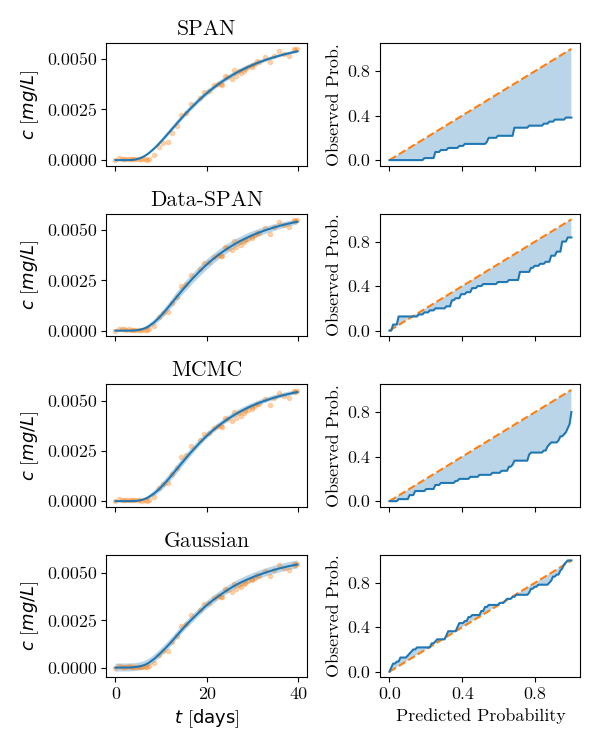
\includegraphics{figs/reliability_curves.png}
    \caption{Top: Core 2 BTC 90\% PIs for the different methods (SPAN, Data-SPAN, MCMC). Bottom: Reliability curve for each method.}
    \label{fig:reliability_curves}
\end{figure}


\subsection{Sensitivity Analysis}
\label{sec:sensitivity}
Sensitivity analysis investigates how variations in input parameters affect the model output. Unweighted SPAN samples inherently perform sensitivity analysis because each sample represents a different set of hyperparameters, and the resulting retardation factor and its impact on the concentration field demonstrate the influence of those hyperparameters.

One sensitivity analysis method is based on standardized regression coefficients, sometimes referred to as beta coefficients or beta weights. They represent the relative importance of each predictor variable (hyperparameter $h$ in this case) in explaining the variance of the outcome variable ($R(c)$).
Importantly, the sum of these normalized coefficients can exceed 1 as parameters may explain common variances. The value shows how important the respective parameter is in relation to the rest.
Since these parameters are based on linear regression, they should be interpreted with caution, especially when non-linear relationships exist between the hyperparameters and the retardation factor.

We average the importance for $R(c)$ over a set of $c$ values and obtain $0.033$ for \textbf{Physical Loss Factor}, $0.051$ for \textbf{Weight Initialization}, $0.159$ for \textbf{MSE Loss Factor}, and $0.570$ for \textbf{Max Epochs}.

This indicates that \textbf{Max Epochs} and \textbf{MSE Loss Factor} have the largest impact on $R(c)$ overall. The seed used for weight initialization and the physical loss factor play only negligible roles.

Figure ~\vref{fig:sensitivity} shows the relative importance for values of $c$ over which the average was taken.


\begin{figure}[h]
    \centering
    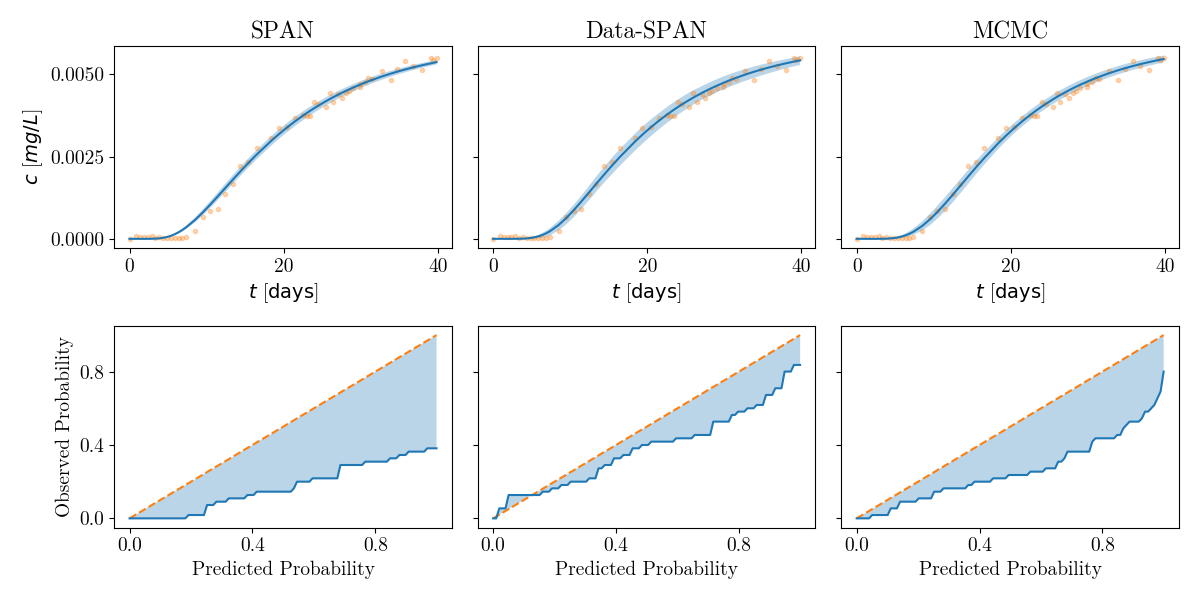
\includegraphics{figs/sensitivity.png}
    \caption{Relative importance on the variance of $R(c)$ of each hyperparameter for different values of $c$.}
    \label{fig:sensitivity}
\end{figure}



\section{Discussion}
\subsection{Retardation Range} % TODO: better name?
For some $c$ $R(c)$ does not affect the whole $c$ field equally. This can be seen by looking at Figure ~\vref{fig:triangle_ret_pertubation} which shows constant retardation curves that are pertubed additively by triangle functions with centers at different $c$ values. With increasing $c$ center, the error caused by the hat functions goes quickly to zero. For $c > 1$, the error becomes zero. This is because the concentration field $c(x,t)$ only contains values between $0$ and $1$. But there is also a noticeable difference between the maximum error measured on the full field vs. the BTC. The BTC error is consistently much lower.
The full field error can not be detected in the case of experimental data as there is no access to the full field solution. For this reason, the range of $c$ values for which significant statements about the uncertainty of $R(c)$ can be made, is restricted to a narrow range. The exact range is difficult to estimate as the stength of influence for different retardations is unclear.


\begin{figure}[h]
    \centering
    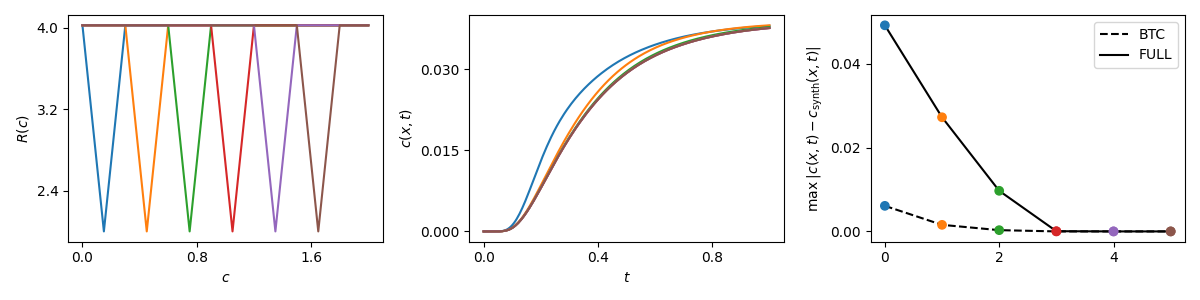
\includegraphics{figs/triangle_ret_pertubation.png}
    \caption{Left: Retardations with triangle peaks. Middle: Concentration BTC for these Retardations. Right: MAE for each on the full field and BTC.}
    \label{fig:triangle_ret_pertubation}
\end{figure}


\subsection{Samples and Prediction Intervals}
The analysis of our results reveals several key insights regarding the performance and characteristics of the different uncertainty estimation methods, particularly focusing on the comparison between Full-SPAN and MCMC.

Firstly, the synthetic data case exhibits significantly lower uncertainty compared to the experimental data scenario. This can be attributed to several factors: a larger number of datapoints, which reduces epistemic uncertainty; the reduced effectiveness of Data-SPAN due to the absence of noise in the synthetic data; and the utilization of less effective SPAN hyperparameters (such as excluding the strongest options like \textbf{Max Epoch} or \textbf{MSE loss factor}, as shown in Section ~\vref{sec:sensitivity}).

Interestingly, Data-SPAN does not demonstrate a substantial improvement in uncertainty estimation with an increasing number of samples, especially when compared to MCMC. This is a favorable characteristic, as it implies that Data-SPAN can achieve reliable uncertainty estimates even with a limited number of samples and thus computational effort. Furthermore, SPAN benefits from trivial parallelizability, unlike MCMC, which requires sequential sampling or more advanced methods. This, coupled with Data-SPAN's ability to operate effectively with fewer samples, establishes SPAN as a more computationally efficient method for UQ.
% TODO: I don't like how I sometimes use SPAN but mean Full-SPAN and stuff like this. Maybe I should introduce Para-SPAN and get rid of Full-SPAN?
% TODO: Btw, I remember that I was told not to use the word "parameter" because this can be confused with something else.

Although our sensitivity analysis indicated that certain hyperparameters exerted minimal influence on the results, their inclusion does not negatively impact performance. This is because Monte Carlo sampling, the core technique employed here, is inherently independent of dimensionality.

Finally, a comparison of the PIs generated by Full-SPAN and MCMC, specifically the $R(c)$ PI, and their respective likelihoods, reveals comparable performance. Qualitatively, both methods appear to achieve a similar level of accuracy in capturing uncertainty.




\subsection{Limitations}
One limitation of our approach lies in its ``brute-force'' nature, due not only to the computational effort but also to the process itself. While we gain insights into uncertainty, the obtained result is highly dependent on the used solver and selected hyperparameters in the case of SPAN and highly depdendent on the given dataset in the case of Data-SPAN. Ideally, uncertainty is a byproduct of the method and the uncertainty in the data.

Furthermore, the weighting process raises concerns. The BTC is constrained to a small subset of concentration values compared to the entire field (only 0 to 0.04 instead of 0 to 1.0). This raises questions about the validity of weighting, e.g. $R(c=0.0)$ samples the same way as $R(c=1.0)$, as the latter do not directly influence the predicted BTC and thus their likelihood contribution is questionable.


\section{Conclusion}
\subsection{Summary}
This work investigated UQ for the retardation factor in a diffusion-sorption process using the FINN framework. We proposed two novel UQ methods, SPAN and Data-SPAN, based on perturbing hyperparameters and training data, respectively. Empirical analysis demonstrated the near-uniqueness of the inverse problem, enabling the interpretation of the UQ results. While computationally more expensive than MCMC, our methods offer a different perspective on uncertainty by directly exploring the effects of various uncertainties within the training data and solver process.

\subsection{Future Work}
% TODO



% TODO: I computed the likelihood also with a gaussian PI. I should also plot this Gaussian PI - maybe even with the reliability curve together.
% TODO: replace .png with .pdf



% TODO: Include this in experiments section
\begin{figure}[h]
    \centering
    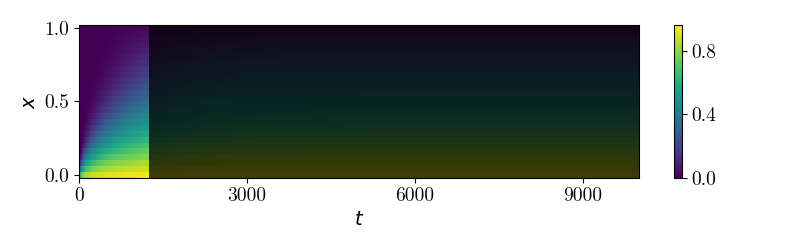
\includegraphics{figs/c_diss_field_full_black_test.png}
    \caption{Training data for the model, represented by a pcolor plot of the synthetic concentration field $c(x,t)$ generated using the Langmuir isotherm. The spatial domain is $x \in [0, 1]$ meters, and the temporal domain is $t \in [0, 10000]$ days. The period from $t = 1255$ to $t = 10000$ days is masked, indicating that these values are not used for training but are reserved for testing.}
    \label{fig:c_diss_field_full_black_test}
\end{figure}